\chapter{Caso de Estudio} \label{Caso de Estudio}

En esta sección se muestra un ejemplo de un caso de uso de la herramienta. Se mostrará tanto el modelo generado de una realidad planteada, como la salida generada de dicho modelo, explicando los detalles de los elementos y su resultado.

Para el caso de estudio se utilizó el diagrama de las Figuras  \ref{fig:caso_estudio} \ref{fig:caso_estudio_pc}, y \ref{fig:caso_estudio_servers}. Este consiste de dos Routers conectados entre sí, por un lado se tiene la subred correspondiente a las PCs, y por otro lado se tienen los Servidores. En la subred de las PCs se tienen dos Switches que separan las computadoras con sistema operativo Unix (y una impresora), de las computadoras Windows. En el lado de los servidores se encuentra un Switch y dichos Servidores.

\begin{figure}[htbp]
    \centering
    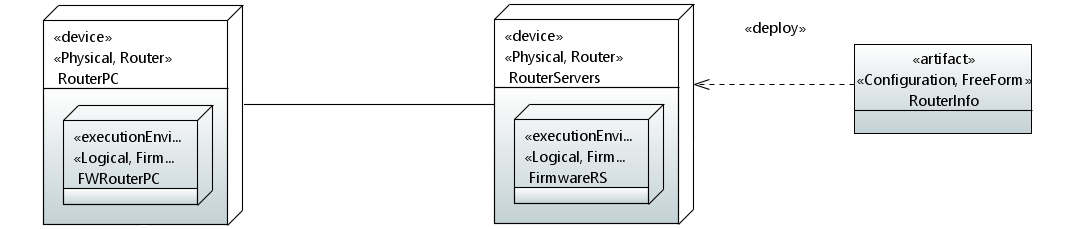
\includegraphics[width=\textwidth]{figures/caso_estudio/study_case_c.png}
    \caption{Ejemplo para el Caso de Estudio (alto nivel).}
    \label{fig:caso_estudio}
\end{figure}

\begin{figure}[htbp]
    \centering
    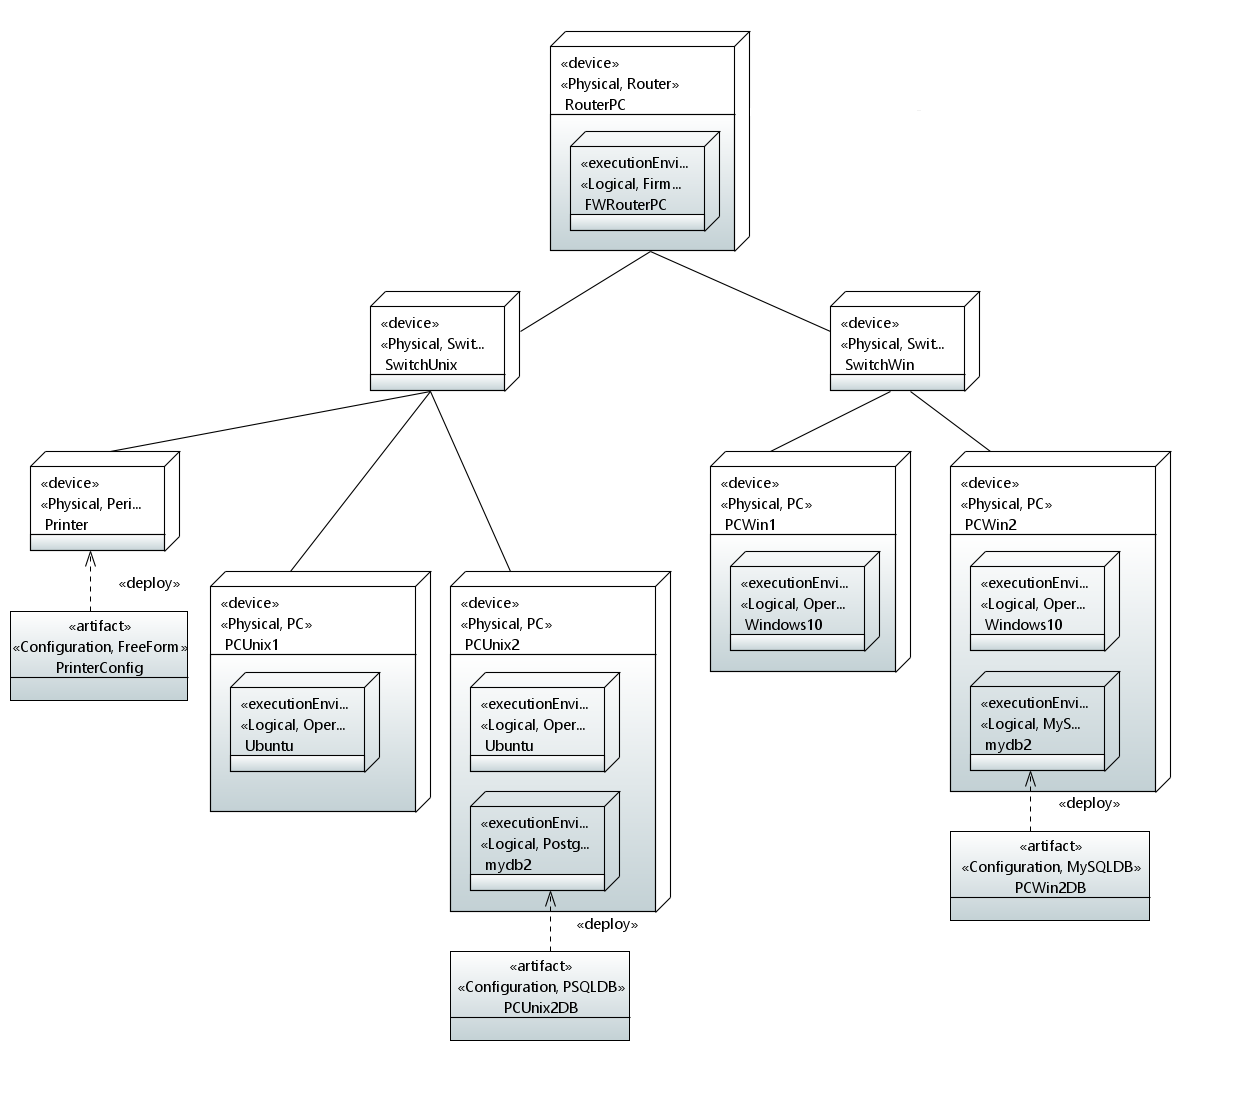
\includegraphics[width=\textwidth]{figures/caso_estudio/study_case_a.png}
    \caption{Ejemplo para el Caso de Estudio - RouterPC.}
    \label{fig:caso_estudio_pc}
\end{figure}

\begin{figure}[htbp]
    \centering
    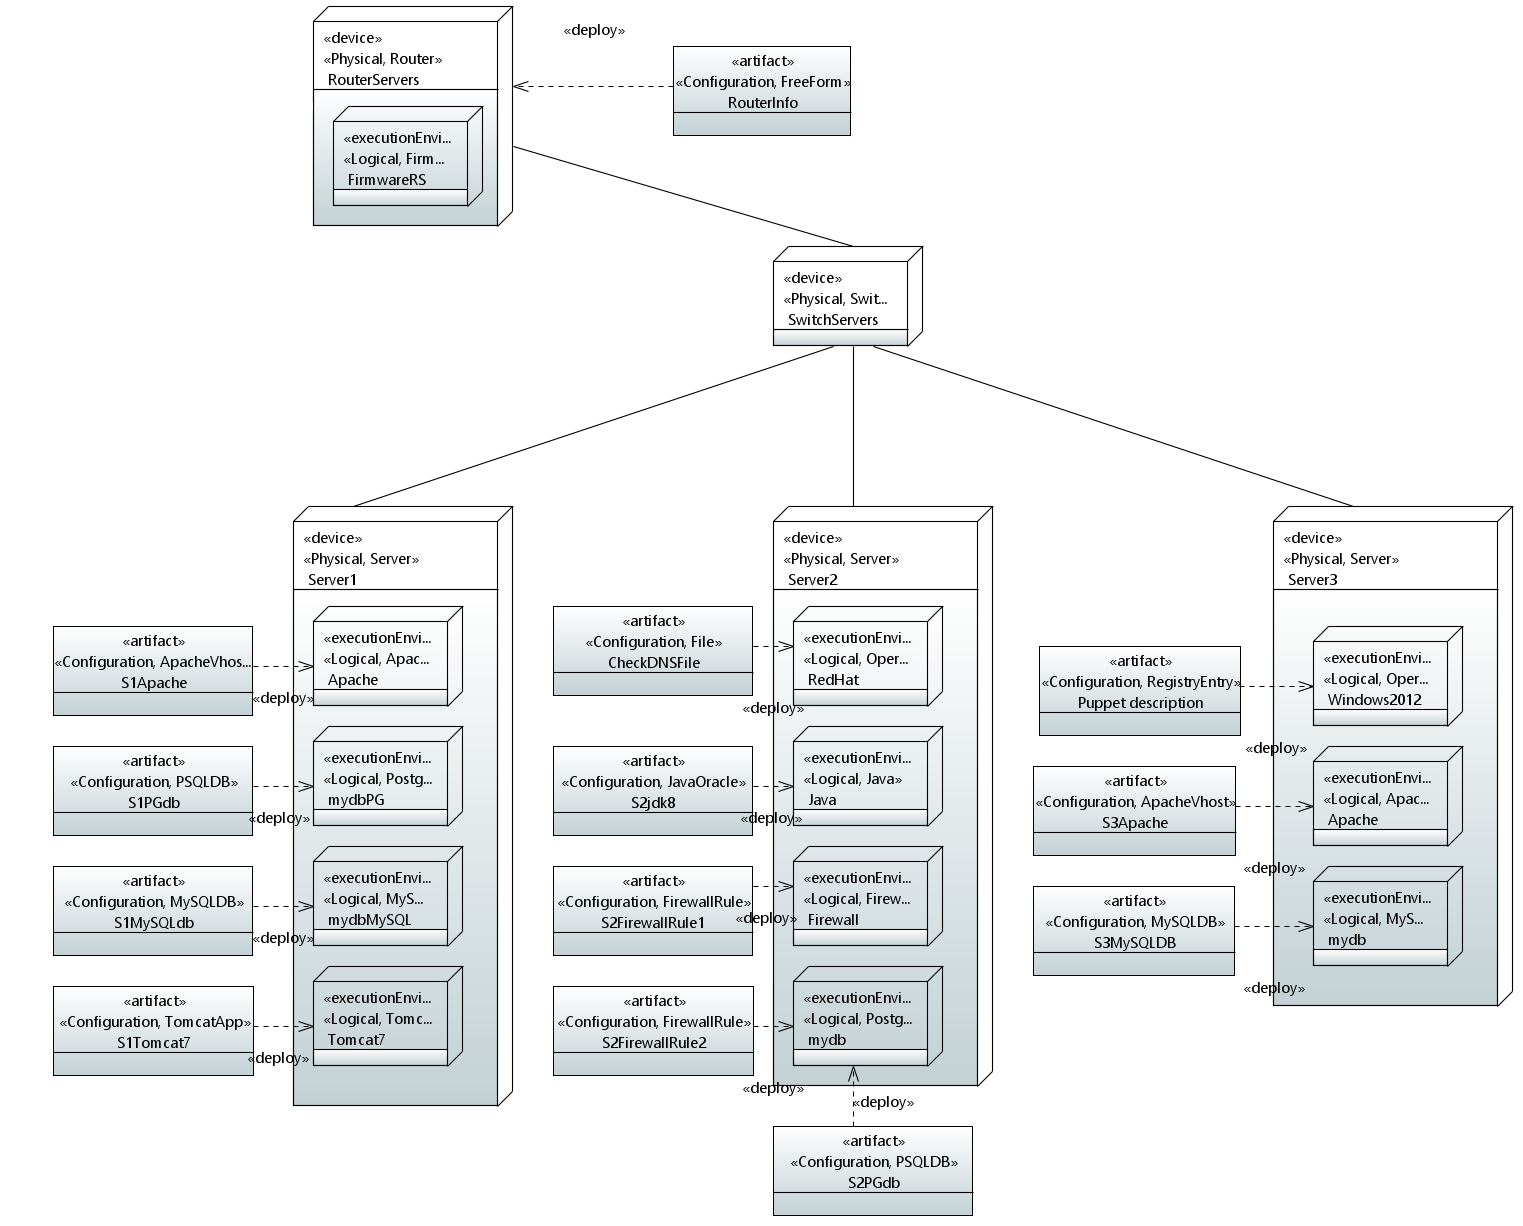
\includegraphics[width=\textwidth]{figures/caso_estudio/study_case_b.png}
    \caption{Ejemplo para el Caso de Estudio - RouterServers.}
    \label{fig:caso_estudio_servers}
\end{figure}

En la figura \ref{fig:caso_estudio:estructura} se pueden observar las
estructuras de archivos generadas por la ejecución de ambas
transformaciones a partir de este diagrama. Como se puede ver, por una
parte se tiene el archivo \textbf{manifests/site.pp}, el archivo
\textbf{Puppetfile} y los directorios \textbf{modules/device} y
\textbf{modules/configurations}, y por otra los directorios
\textbf{Configurations} e \textbf{Information}. Dentro del directorio
\textbf{modules/device} se encuentra un archivo de configuración por
cada componente del tipo \textbf{Device} que sea configurable, y
además su correspondiente directorio. Dentro del directorio
\textbf{modules/configurations}, se encuentra un directorio por cada
clase de componente que se encuentra en el diagrama, esta distribución
permite identificar fácilmente las diferentes clases de componentes
lógicos. También se encuentra el directorio \textbf{Configurations} que
contiene configuración del tipo \textbf{Libre} para cada
componente. Por último se tiene el directorio \textbf{Information},
que contiene un directorio por cada componente de tipo
\textbf{Device}, es decir cada componente físico, presente en el
diagrama. Como es de esperar, estos directorios estarán presentes con
la condición de que exista su respectivo componente en el diagrama.

\begin{figure}[htbp]
    \centering
    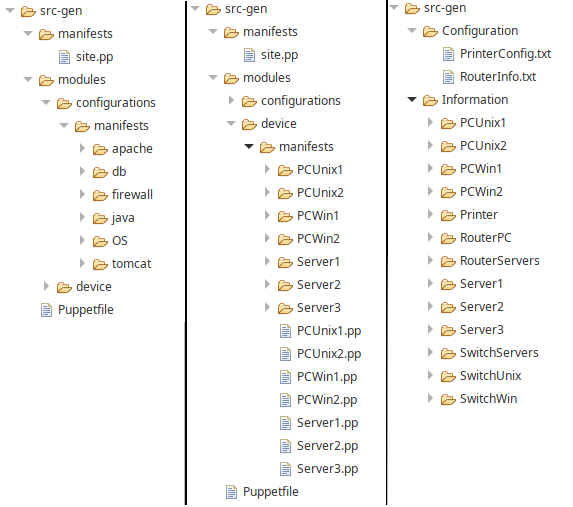
\includegraphics[width=0.80\textwidth]{figures/caso_estudio/estructura.png}
    \caption{Estructura de archivos generada para el Caso de Estudio.}
    \label{fig:caso_estudio:estructura}
\end{figure}

Teniendo presente la estructura de directorios generada, se puede pasar a analizar elementos en particular, y el resultado de la transformación generada. En la Figura \ref{fig:caso_estudio:ejemplo_pcunix2} se tiene el componente de clase \textbf{device} \textbf{PCUnix2}, dicho componente tiene a su vez dos nodos \textbf{lógicos}, y existe un artefacto \textbf{configuration} aplicado a uno de estos nodos. Al ejecutar la transformación mdcms2puppet esto generará el archivo \textbf{PCUnix2.pp}, y un directorio con el mismo nombre, ubicado bajo el directorio \textbf{modules/device/manifests}. Al mismo tiempo, en el directorio \textbf{PCUnix2} se generará un archivo por cada nodo lógico presente, en este caso dos: \textbf{mydb2.pp} y \textbf{Ubuntu.pp} (dado que los componentes se crearon con estos nombres). Esta estructura se puede ver en la Figura \ref{fig:caso_estudio:ejemplo_pcunix2_gen}.
Luego, dado que se tiene un artefacto \textbf{configuration} de tipo \textbf{PSQLDB}, se creará bajo el directorio \textbf{/modules/configurations/manifests/db} un archivo con el nombre de dicho artefacto, en este caso \textbf{PCUnix2DB}, conteniendo la configuración de la base de datos.
Al ejecutar la transformación mdcms2info, dentro del directorio \textbf{information} y bajo el directorio con su nombre (\textbf{PCUnix2}), se creará un archivo correspondiente al device (en este caso \textbf{PC}), y otro correspondiente al sistema operativo, con los nombres de dichos componentes. Los archivos de información se crearán dependiendo del componente, dado que sólo los que contienen información relevante serán creados (como se explicó en secciones previas).
En la Figura \ref{fig:caso_estudio:ejemplo_pcunix2_gen} se pueden ver resaltados los archivos generados a partir del componente en la Figura \ref{fig:caso_estudio:ejemplo_pcunix2}.

\begin{figure}[htbp]
    \centering
    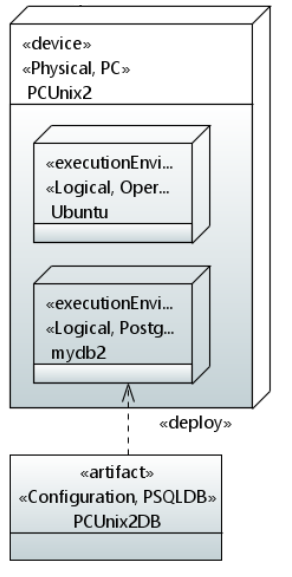
\includegraphics[width=0.25\textwidth]{figures/caso_estudio/ej_pcunix2.png}
    \caption{Componente de ejemplo PCUnix2.}
    \label{fig:caso_estudio:ejemplo_pcunix2}
\end{figure}

\begin{figure}[htbp]
    \centering
    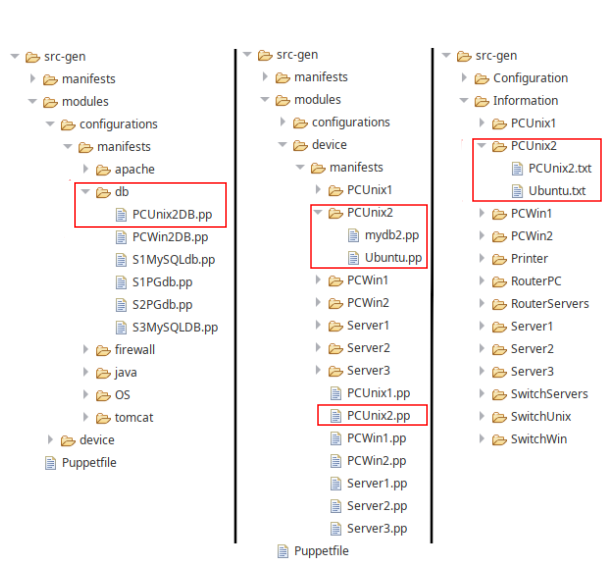
\includegraphics[width=0.8\textwidth]{figures/caso_estudio/ej_pcunix2_gen.png}
    \caption{Archivos generados a partir de la transformación del componente PCUnix2.}
    \label{fig:caso_estudio:ejemplo_pcunix2_gen}
\end{figure}

Conociendo la estructura de directorios y los archivos generados, se puede pasar a analizar el contenido de estos archivos. En primer lugar se tiene el archivo principal \textbf{manifests/site.pp}, el cual se encarga de declarar los componentes que se definieron, incluyendo el nodo de ejemplo \textbf{PCUnix2}, como se puede ver en la Figura \ref{fig:caso_estudio:site_pp}.

\begin{figure}[htbp]
    \centering
    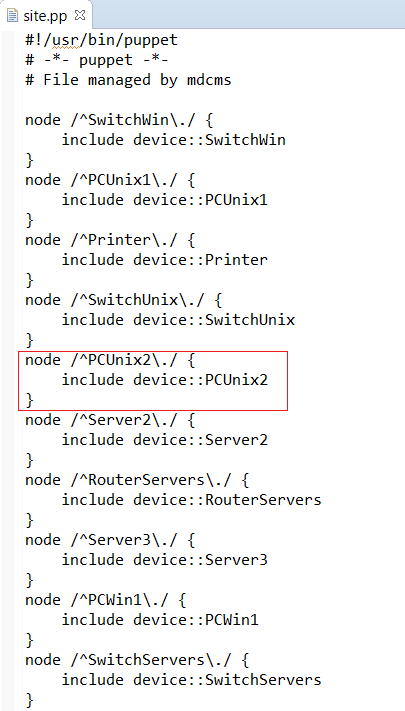
\includegraphics[width=0.5\textwidth]{figures/caso_estudio/site_pp.png}
    \caption{Declaración de nodos en el archivo Site.pp.}
    \label{fig:caso_estudio:site_pp}
\end{figure}

Luego, se tienen los archivos de definición de cada nodo en particular bajo el directorio \textbf{modules/device/manifests}, en este caso tenemos el archivo base \textbf{PCUnix2.pp} que se encarga de incluir los componentes lógicos definidos, y sus dos archivos correspondientes, \textbf{mydb2.pp}, y \textbf{Ubuntu.pp}. Dichos archivos definen los componentes con los parámetros indicados, en caso de que el componente sea configurable. Los atributos utilizados en los componentes de \textbf{PCUnix2} se pueden ver en las Figuras \ref{fig:caso_estudio:pcunix2_prop}, \ref{fig:caso_estudio:ubuntu_prop}, \ref{fig:caso_estudio:mydb2_prop}, mientras que los archivos generados tendrán la forma que se muestra en la Figura \ref{fig:caso_estudio:pcunix2_device}.

\begin{figure}[htbp]
    \centering
    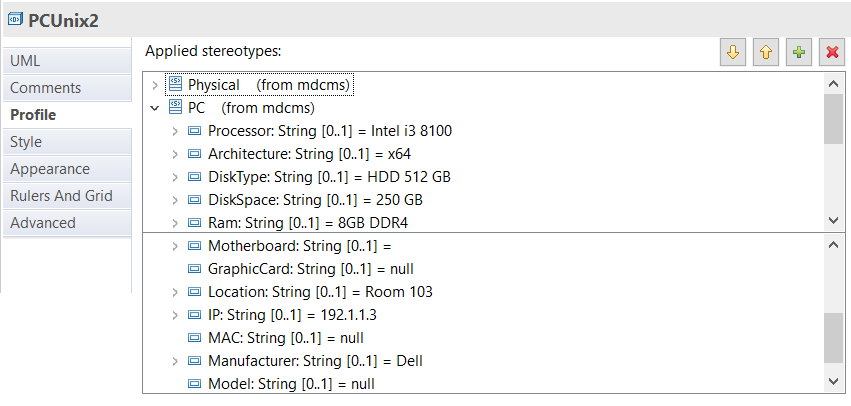
\includegraphics[width=0.8\textwidth]{figures/caso_estudio/pcunix2_properties.png}
    \caption{Propiedades del componente PCUnix2.}
    \label{fig:caso_estudio:pcunix2_prop}
\end{figure}

\begin{figure}[htbp]
    \centering
    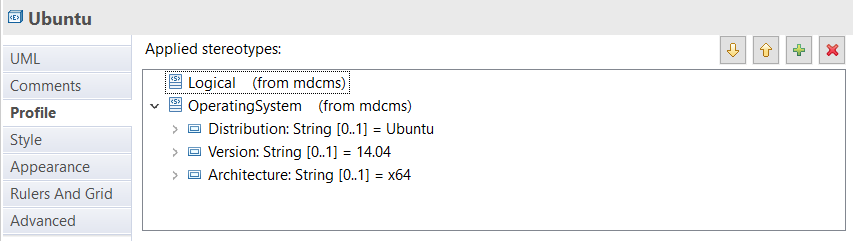
\includegraphics[width=0.8\textwidth]{figures/caso_estudio/ubuntu_properties.png}
    \caption{Propiedades del nodo lógico Ubuntu de PCUnix2.}
    \label{fig:caso_estudio:ubuntu_prop}
\end{figure}

\begin{figure}[htbp]
    \centering
    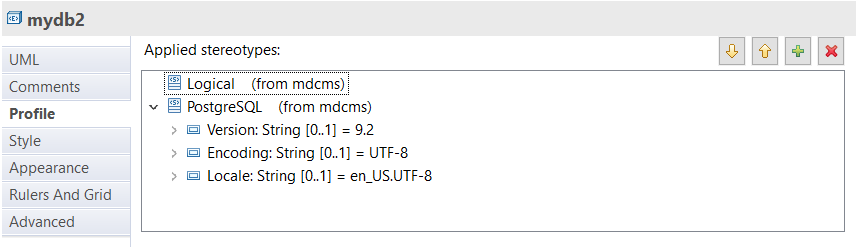
\includegraphics[width=0.8\textwidth]{figures/caso_estudio/mydb2_properties.png}
    \caption{Propiedades del nodo lógico mydb2 de PCUnix2.}
    \label{fig:caso_estudio:mydb2_prop}
\end{figure}

\begin{figure}[htbp]
    \centering
    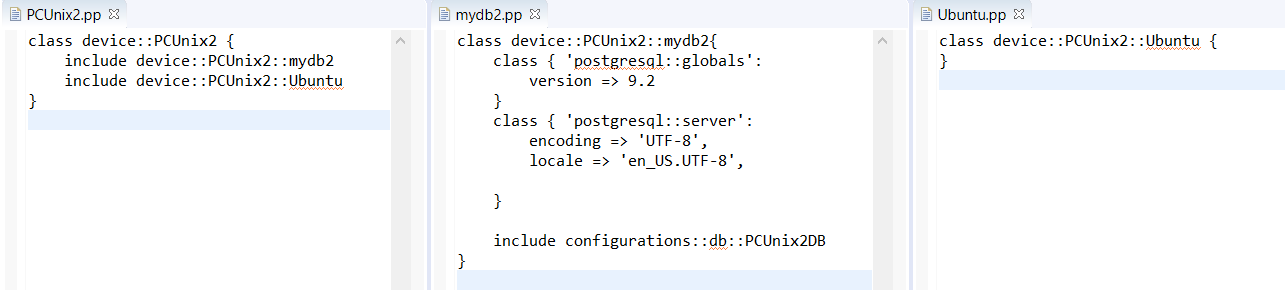
\includegraphics[width=\textwidth]{figures/caso_estudio/ej_pcunix2_device.png}
    \caption{Archivos generados a partir de los componentes lógicos de PCUnix2.}
    \label{fig:caso_estudio:pcunix2_device}
\end{figure}

En el lado de la configuración, tenemos el artefacto \textbf{PCUnix2DB} aplicado al nodo lógico \textbf{mydb2}, que a su vez esta instalado en el nodo físico \textbf{PCUnix2}. Las propiedades de dicho artefacto se pueden ver en la Figura \ref{fig:caso_estudio:pcunix2db_prop}, mientras que el archivo de configuración generado se encuentra en la Figura \ref{fig:caso_estudio:pcunix2db_gen}. Como referencia, en la Figura \ref{fig:caso_estudio:puppet_psql} se incluye un ejemplo simple de una configuración de este componente (Postgresql) utilizando Puppet, tomado de la definición del componente en la página web de Puppet. \cite{puppet_psql}

\begin{figure}[htbp]
    \centering
    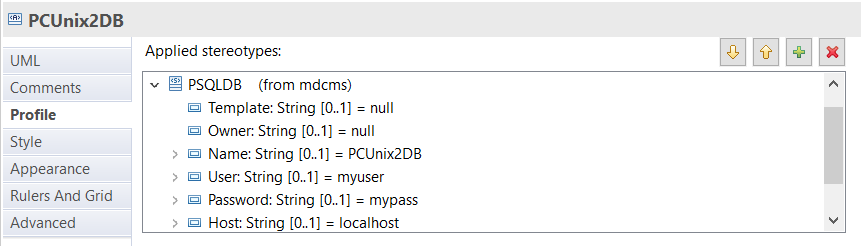
\includegraphics[width=0.8\textwidth]{figures/caso_estudio/pcunix2db_properties.png}
    \caption{Propiedades del artefacto PCUnix2DB aplicado al nodo lógico mydb2 de PCUnix2.}
    \label{fig:caso_estudio:pcunix2db_prop}
\end{figure}

\begin{figure}[htbp]
    \centering
    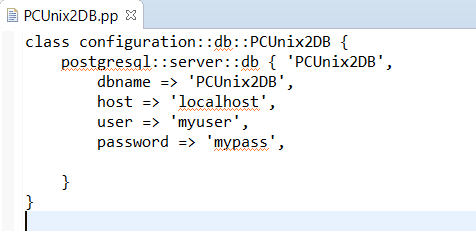
\includegraphics[width=0.5\textwidth]{figures/caso_estudio/pcunix2db_gen.png}
    \caption{Archivo de configuración generado para el artefacto PCUnix2DB.}
    \label{fig:caso_estudio:pcunix2db_gen}
\end{figure}

\begin{figure}[htbp]
    \centering
    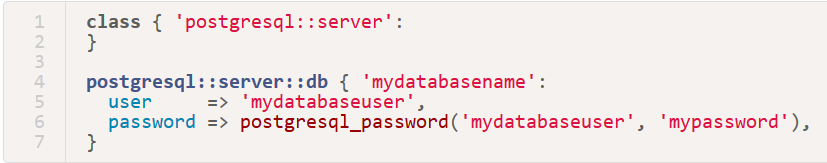
\includegraphics[width=0.8\textwidth]{figures/caso_estudio/puppet_psql.png}
    \caption{Archivo de configuración para PSQL en Puppet.}
    \label{fig:caso_estudio:puppet_psql}
\end{figure}

Por último tenemos los archivos de información generados para el componente \textbf{PCUnix2}, y su sistema operativo \textbf{Ubuntu}, las propiedades de dichos componentes se pueden ver en las Figuras \ref{fig:caso_estudio:pcunix2_prop} y \ref{fig:caso_estudio:ubuntu_prop} respectivamente. Los archivos de información que se generen dependerán de la clase de componentes que se definan en el modelo, dado que se generan únicamente para aquellos que sean relevantes, como se explicó previamente. Los archivos generados para los componentes mencionados anteriormente se pueden apreciar en la Figura \ref{fig:caso_estudio:pcunix2_info_gen}.

\begin{figure}[htbp]
    \centering
    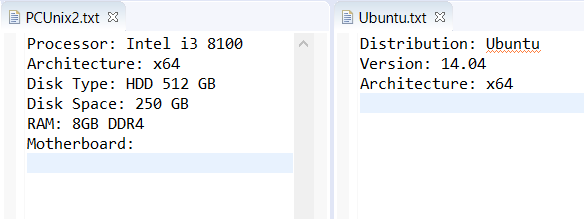
\includegraphics[width=0.8\textwidth]{figures/caso_estudio/pcunix2_info_gen.png}
    \caption{Archivos de información generados para los componentes PCUnix2 y Ubuntu.}
    \label{fig:caso_estudio:pcunix2_info_gen}
\end{figure}

%%% Local Variables:
%%% TeX-master: "../main"
%%% End:
